\section{Thesis Outline} \label{sec:thesis-outline}

This thesis is structured into five chapters.

\Cref{sec:introduction} introduces and motivates the problem of finding relevant research papers in a growing body of scientific literature, highlighting the need for an automated, reliable and precise paper recommender system (\Cref{sec:problem-statement-motivation}). It then presents the research objective and its derived research tasks (\Cref{sec:research-objectives}) and outlines the structure of the thesis (\Cref{sec:thesis-outline}).

\Cref{sec:background-related-work} reviews the existing literature on paper recommender systems and provides foundational knowledge for the subsequent chapters. It begins with a broad overview of general recommender systems, detailing their different types and common evaluation strategies (\Cref{sec:recommender-systems}). Following this, \Cref{sec:citation-analysis} explores how citation-based methods are used in recommender systems. \Cref{sec:semantic-analysis} then discusses content-based approaches, with a particular focus on language models that use the semantic information of documents. Lastly, \Cref{sec:hybrid-recommenders-for-academic-papers} summarizes the current work on hybrid recommender systems for academic papers and highlights this thesis's contributions.

\Cref{sec:methodology} describes the methodology used to develop the hybrid recommender system. First, a conceptual overview of the system is given (\Cref{sec:overview}). Then, the data sources for this thesis and the dataset construction process are presented (\Cref{sec:dataset-construction}). Next, detailed information on the training or precomputation phase (\Cref{sec:training}) and the inference phase (\Cref{sec:inference}) is provided.

\Cref{sec:evaluation} evaluates the hybrid recommender system. First, \Cref{sec:evaluation-strategy} introduces the systematic and data-driven evaluation strategy of this thesis.
Then, the results of the evaluation are presented by identifying the bibliographic coupling score as the most influential feature for the Citation Recommender, SciBERT as the most effective language model for the Language Recommender, and the \ac{L2C} hybridization order as superior to the \ac{C2L} order (\Cref{sec:evaluation-results}).

Finally, \Cref{sec:conclusion} concludes the thesis by summarizing the methodology and findings (\Cref{sec:summary}).
\Cref{sec:broader-impact} highlights the contributions of this thesis to the broader field of paper recommender systems, while \Cref{sec:outlook} points out current limitations and starting points for future work.

\Cref{fig:thesis-outline} illustrates the thesis structure graphically.

\begin{figure}[htb!]
    \centering
    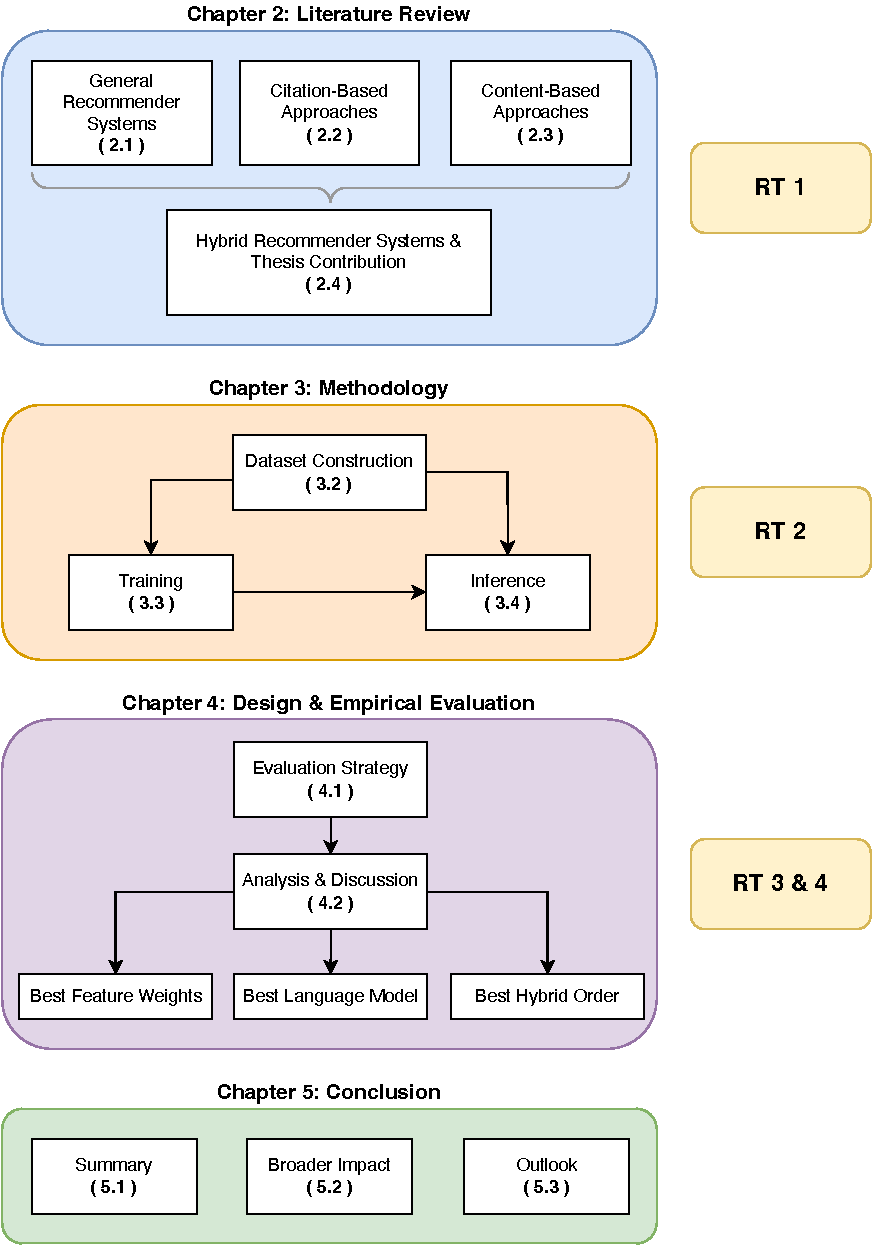
\includegraphics[width=0.8\textwidth]{diagrams/thesis_outline.pdf}
    \caption[Thesis Structure]{Thesis structure visualized. The diagram is adapted from \cite{BreitingerAcademicLiterature2023}.
        \textbf{\ac{RT} 1} - \textbf{\ac{RT} 4} derived in \Cref{sec:research-objectives} are added to their respective chapters.}
    \label{fig:thesis-outline}
\end{figure}